
\chapter{Decision Trees} \label{sec:dt}

\chapterquote{The words printed here are concepts.\\You must go through the experiences.}{Carl~Frederick}


%\chapterimageopt{serious.png}{width=5cm}{Courtesy XKCD}

\begin{learningobjectives}
\item Explain the difference between memorization and generalization.
\item Define ``inductive bias'' and recognize the role of inductive
  bias in learning.
\item Take a concrete task and cast it as a learning problem, with a
  formal notion of input space, features, output space, generating
  distribution and loss function.
\item Illustrate how regularization trades off between underfitting
  and overfitting.
\item Evaluate whether a use of test data is ``cheating'' or not.
\end{learningobjectives}

\dependencies{None.}

\newthought{At a basic level,} machine learning is about predicting
the future based on the past.  For instance, you might wish to predict
how much a user Alice will like a movie that she hasn't seen, based on
her ratings of movies that she has seen.  This means making informed
guesses about some unobserved property of some object, based on
observed properties of that object.

The first question we'll ask is: what does it mean to learn?  In order
to develop learning machines, we must know what learning actually
means, and how to determine success (or failure).  You'll see this
question answered in a very limited learning setting, which will be
progressively loosened and adapted throughout the rest of this book.
For concreteness, our focus will be on a very simple model of learning
called a \concept{decision tree}.

\begin{vignette}{Alice Decides which Classes to Take}
todo
\end{vignette}


\section{What Does it Mean to Learn?}

Alice has just begun taking a course on machine learning.  She knows
that at the end of the course, she will be expected to have ``learned''
all about this topic.  A common way of gauging whether or not she has
learned is for her teacher, Bob, to give her a exam.  She has done
well at learning if she does well on the exam.

But what makes a reasonable exam?  If Bob spends the entire semester
talking about machine learning, and then gives Alice an exam on
History of Pottery, then Alice's performance on this exam will
\emph{not} be representative of her learning.  On the other hand, if
the exam only asks questions that Bob has answered exactly during lectures,
then this is also a bad test of Alice's learning, especially if it's
an ``open notes'' exam.  What is desired is that Alice observes
\emph{specific} examples from the course, and then has to answer new, but
related questions on the exam.  This tests whether Alice has the
ability to \concept{generalize}.  Generalization is perhaps the most
central concept in machine learning.

As a running concrete example in this book, we will use that of a
course recommendation system for undergraduate computer science
students.  We have a collection of students and a collection of
courses.  Each student has taken, and evaluated, a subset of the
courses.  The evaluation is simply a score from $-2$ (terrible) to
$+2$ (awesome).  The job of the recommender system is to
\concept{predict} how much a particular student (say, Alice) will like
a particular course (say, Algorithms).

Given historical data from course ratings (i.e., the past) we are
trying to predict unseen ratings (i.e., the future).  Now, we could be
unfair to this system as well.  We could ask it whether Alice is
likely to enjoy the History of Pottery course.  This is unfair because
the system has no idea what History of Pottery even is, and has no
prior experience with this course.  On the other hand, we could ask it
how much Alice will like Artificial Intelligence, which she took last
year and rated as $+2$ (awesome).  We would expect the system to
predict that she would really like it, but this isn't demonstrating
that the system has learned: it's simply recalling its past
experience.  In the former case, we're expecting the system to
generalize \emph{beyond} its experience, which is unfair.  In the
latter case, we're not expecting it to generalize at all.

This general set up of predicting the future based on the past is at
the core of most machine learning.  The objects that our algorithm
will make predictions about are \concept{examples}.  In the
recommender system setting, an example would be some particular
Student/Course pair (such as Alice/Algorithms).  The desired
prediction would be the rating that Alice would give to Algorithms.

%\TODOFigure{dt:induction}{A figure showing training data to a
%  ML algorithm to a function $f$ and then predictions on test data.}

\Figure{dt:induction}{The general supervised approach to machine
  learning: a learning algorithm reads in training data and computes a
  learned function $f$.  This function can then automatically label
  future text examples.}

To make this concrete, Figure~\ref{fig:induction} shows the general
framework of \concept{induction}.  We are given \concept{training
  data} on which our algorithm is expected to learn.  This training
data is the examples that Alice observes in her machine learning
course, or the historical ratings data for the recommender system.
Based on this training data, our learning algorithm induces a function
$f$ that will map a new example to a corresponding prediction.  For
example, our function might guess that $f(\text{Alice/Machine
  Learning})$ might be high because our training data said that Alice
liked Artificial Intelligence.  We want our algorithm to be able to
make lots of predictions, so we refer to the collection of examples on
which we will evaluate our algorithm as the \concept{test set}.  The
test set is a closely guarded secret: it is the final exam on which
our learning algorithm is being tested.  If our algorithm gets to peek
at it ahead of time, it's going to cheat and do better than it should.

\thinkaboutit{Why is it bad if the learning algorithm gets to peek at the test data?}

The goal of inductive machine learning is to take some training data
and use it to induce a function $f$.  This function $f$ will be
evaluated on the test data.  The machine learning algorithm has
succeeded if its performance on the test data is high.

\section{Some Canonical Learning Problems}

There are a large number of typical inductive learning problems.  The
primary difference between them is in what type of \emph{thing}
they're trying to predict.  Here are some examples:

\begin{description}
\item[Regression:] trying to predict a real value.  For instance,
  predict the value of a stock tomorrow given its past performance.
  Or predict Alice's score on the machine learning final exam based on
  her homework scores.

\item[Binary Classification:] trying to predict a simple yes/no
  response.  For instance, predict whether Alice will enjoy a course
  or not.  Or predict whether a user review of the newest Apple
  product is positive or negative about the product.

\item[Multiclass Classification:] trying to put an example into one of
  a number of classes.  For instance, predict whether a news story is
  about entertainment, sports, politics, religion, etc.  Or predict
  whether a CS course is Systems, Theory, AI or Other.

\item[Ranking:] trying to put a set of objects in order of relevance.
  For instance, predicting what order to put web pages in, in response
  to a user query.  Or predict Alice's ranked preferences over courses
  she hasn't taken.
\end{description}

\thinkaboutit{For each of these types of canonical machine learning
  problems, come up with one or two concrete examples.}

The reason that it is convenient to break machine learning problems
down by the type of object that they're trying to predict has to do
with measuring error.  Recall that our goal is to build a system that
can make ``good predictions.''  This begs the question: what does it
mean for a prediction to be ``good?''  The different types of learning
problems differ in how they define goodness.  For instance, in
regression, predicting a stock price that is off by $\$0.05$ is
perhaps much better than being off by $\$200.00$.  The same does not
hold of multiclass classification.  There, accidentally predicting
``entertainment'' instead of ``sports'' is no better or worse than
predicting ``politics.''


%TODO? what have they heard of that does ML?  what haven't they heard of?

%batch versus online learning

\section{The Decision Tree Model of Learning}

The \concept{decision tree} is a classic and natural model of
learning.  It is closely related to the fundamental computer science
notion of ``divide and conquer.''  Although decision trees can be
applied to many learning problems, we will begin with the simplest
case: binary classification.

Suppose that your goal is to predict whether some unknown user will
enjoy some unknown course.  You must simply answer ``yes'' or ``no.''
In order to make a guess, your're allowed to ask binary questions
about the user/course under consideration.  For example:

{\bf You:} Is the course under consideration in Systems?\\
{\bf Me:}  Yes\\
{\bf You:} Has this student taken any other Systems courses?\\
{\bf Me:}  Yes\\
{\bf You:} Has this student like most previous Systems courses?\\
{\bf Me:}  No\\
{\bf You:} \emph{I predict this student will not like this course.}\\

The goal in learning is to figure out what questions to ask, in what
order to ask them, and what answer to predict once you have asked
enough questions.

%\TODOFigure{dt:example}{A simple picture of a decision tree for course recommendation, consistent with the text example.}

\MoveNextFigure{-10cm}
\Figure{dt:example}{A decision tree for a course recommender system,
  from which the in-text ``dialog'' is drawn.}

The decision tree is so-called because we can write our set of
questions and guesses in a tree format, such as that in
Figure~\ref{fig:dt:example}.  In this figure, the questions are
written in the internal tree nodes (rectangles) and the guesses are
written in the leaves (ovals).  Each non-terminal node has two
children: the left child specifies what to do if the answer to the
question is ``no'' and the right child specifies what to do if it is
``yes.''

In order to learn, I will give you training data.  This data consists
of a set of user/course examples, paired with the correct answer for
these examples (did the given user enjoy the given course?).  From
this, you must construct your questions.  For concreteness, there is a
small data set in Table~\ref{tab:data:course} in the Appendix of this
book.  This training data consists of 20 course rating examples, with
course ratings and answers to questions that you might ask about this
pair.  We will interpret ratings of $0$, $+1$ and $+2$ as ``liked'' and
ratings of $-2$ and $-1$ as ``hated.''

In what follows, we will refer to the questions that you can ask as
\concept{features} and the responses to these questions as
\concept{feature values}.  The rating is called the \concept{label}.
An example is just a set of feature values.  And our training data is
a set of examples, paired with labels.

There are a lot of logically possible trees that you could build, even
over just this small number of features (the number is in the
millions).  It is computationally infeasible to consider all of these
to try to choose the ``best'' one.  Instead, we will build our
decision tree \emph{greedily.}  We will begin by asking:

{\bf If I could only ask one question, what question would I ask?}

%\TODOFigure{dt:histogram}{A figure showing the histogram of labels
%  given features for the first four features from the data in the
%  appendix.}

\MoveNextFigure{-10cm}
\Figure{dt:histogram}{A histogram of labels for (a) the entire data
  set; (b-e) the examples in the data set for each value of the first
  four features.}

You want to find a feature that is \emph{most useful} in helping you
guess whether this student will enjoy this course.\sidenote{A
  colleague related the story of getting his 8-year old nephew to
  guess a number between 1 and 100.  His nephew's first four questions
  were: Is it bigger than 20?  (YES) Is it even?  (YES) Does it have a
  7 in it?  (NO) Is it 80?  (NO).  It took 20 more questions to get
  it, even though 10 should have been sufficient.  At 8, the nephew
  hadn't quite figured out how to divide and conquer.
  \url{http://blog.computationalcomplexity.org/2007/04/getting-8-year-old-interested-in.html}.}
A useful way to think about this is to look at the \concept{histogram}
of labels for each feature.  This is shown for the first four features
in Figure~\ref{fig:dt:histogram}.  Each histogram shows the frequency
of ``like''/``hate'' labels for each possible value of an associated
feature.  From this figure, you can see that asking the first feature
is not useful: if the value is ``no'' then it's hard to guess the
label; similarly if the answer is ``yes.''  On the other hand, asking
the second feature \emph{is} useful: if the value is ``no,'' you can
be pretty confident that this student will like this course; if the
answer is ``yes,'' you can be pretty confident that this student will
hate this course.

More formally, you will consider each feature in turn.  You might
consider the feature ``Is this a System's course?''  This feature has
two possible value: no and yes.  Some of the training examples have an
answer of ``no'' -- let's call that the ``NO'' set.  Some of the
training examples have an answer of ``yes'' -- let's call that the
``YES'' set.  For each set (NO and YES) we will build a histogram over
the labels.  This is the second histogram in
Figure~\ref{fig:dt:histogram}.  Now, suppose you were to ask this
question on a random example and observe a value of ``no.''  Further
suppose that you must \emph{immediately} guess the label for this
example.  You will guess ``like,'' because that's the more prevalent
label in the NO set (actually, it's the \emph{only} label in the NO
set).  Alternative, if you recieve an answer of ``yes,'' you will
guess ``hate'' because that is more prevalent in the YES set.

So, for this single feature, you know what you \emph{would} guess if
you had to.  Now you can ask yourself: if I made that guess on the
\emph{training data,} how well would I have done?  In particular, how
many examples would I classify \emph{correctly?}  In the NO set (where
you guessed ``like'') you would classify all $10$ of them correctly.
In the YES set (where you guessed ``hate'') you would classify $8$
(out of $10$) of them correctly.  So overall you would classify $18$
(out of $20$) correctly.  Thus, we'll say that the \emph{score} of the
``Is this a System's course?'' question is $18/20$.

\thinkaboutit{How many training examples would you classify correctly
  for each of the other three features from
  Figure~\ref{fig:dt:histogram}?}

You will then repeat this computation for each of the available
features to us, compute the scores for each of them.  When you must
choose which feature consider first, you will want to choose the one
with the highest score.

But this only lets you choose the \emph{first} feature to ask about.
This is the feature that goes at the \emph{root} of the decision tree.
How do we choose subsequent features?  This is where the notion of
divide and conquer comes in.  You've already decided on your first
feature: ``Is this a Systems course?''  You can now \emph{partition}
the data into two parts: the NO part and the YES part.  The NO part is
the subset of the data on which value for this feature is ``no''; the
YES half is the rest.  This is the \emph{divide} step.

The \emph{conquer} step is to recurse, and run the \emph{same}
routine (choosing the feature with the highest score) on the NO set
(to get the left half of the tree) and then separately on the YES set
(to get the right half of the tree).

At some point it will become useless to query on additional features.
For instance, once you know that this is a Systems course, you
\emph{know} that everyone will hate it.  So you can immediately
predict ``hate'' without asking any additional questions.  Similarly,
at some point you might have already queried every available feature
and still not whittled down to a single answer.  In both cases, you
will need to create a leaf node and guess the most prevalent answer in
the current piece of the training data that you are looking at.


\newalgorithm%
  {dt:train}%
  {\FUN{DecisionTreeTrain}(\VAR{data}, \VAR{remaining features})}%
  {
\SETST{guess} most frequent answer in \VAR{data} \COMMENT{default answer for this data}
\IF{the labels in \VAR{data} are unambiguous}
\RETURN \STR{Leaf}(\VAR{guess}) \COMMENT{base case: no need to split further}
\ELSIF{\VAR{remaining features} is empty}
\RETURN \STR{Leaf}(\VAR{guess}) \COMMENT{base case: cannot split further}
\ELSE[we need to query more features]
\FORALL{\VAR{f} $\in$ \VAR{remaining features}}
\SETST{NO} the subset of \VAR{data} on which \VAR{f}=\CON{no}
\SETST{YES} the subset of \VAR{data} on which \VAR{f}=\CON{yes}
\STATE \VAR{score}[\VAR{f}] $\leftarrow$ \# of majority vote answers in \VAR{NO}
\STATE \quad\quad\quad\quad + \# of majority vote answers in \VAR{YES}\\
\COMMENT{the accuracy we would get if we only queried on \VAR{f}}
\ENDFOR
\SETST{f} the feature with maximal \VAR{score}(\VAR{f})
\SETST{NO} the subset of \VAR{data} on which \VAR{f}=\CON{no}
\SETST{YES} the subset of \VAR{data} on which \VAR{f}=\CON{yes}
\SETST{left} \FUN{DecisionTreeTrain}(\VAR{NO}, \VAR{remaining features} $\without$ $\{$\VAR{f}$\}$)
\SETST{right} \FUN{DecisionTreeTrain}(\VAR{YES}, \VAR{remaining features} $\without$ $\{$\VAR{f}$\}$)
\RETURN \STR{Node}(\VAR{f}, \VAR{left}, \VAR{right})
\ENDIF
}

\newalgorithm%
  {dt:predict}%
  {\FUN{DecisionTreeTest}(\VAR{tree}, \VAR{test point})}
  {
\IF{\VAR{tree} is of the form \STR{Leaf}(\VAR{guess})}
\RETURN \VAR{guess}
\ELSIF{\VAR{tree} is of the form \STR{Node}(\VAR{f}, \VAR{left}, \VAR{right})}
\IF{\VAR{f} $=$ \CON{yes} in \VAR{test point}}
\RETURN \FUN{DecisionTreeTest}(\VAR{left}, \VAR{test point})
\ELSE
\RETURN \FUN{DecisionTreeTest}(\VAR{right}, \VAR{test point})
\ENDIF
\ENDIF
}

Putting this all together, we arrive at the algorithm shown in
Algorithm~\ref{alg:dt:train}.\sidenote{There are more nuanced
  algorithms for building decision trees, some of which are discussed
  in later chapters of this book.  They primarily differ in how they
  compute the \emph{score} funciton.}  This function,
\FUN{DecisionTreeTrain} takes two arguments: our data, and the set of
as-yet unused features.  It has two base cases: either the data is
unambiguous, or there are no remaining features.  In either case, it
returns a \STR{Leaf} node containing the most likely guess at this
point.  Otherwise, it loops over all remaining features to find the
one with the highest score.  It then partitions the data into a NO/YES
split based on the best feature.  It constructs its left and right
subtrees by recursing on itself.  In each recursive call, it uses one
of the partitions of the data, and removes the just-selected feature
from consideration.

\thinkaboutit{Is the Algorithm in Figure~\ref{fig:dt:train}
  guaranteed to terminate?}

The corresponding \emph{prediction} algorithm is shown in
Algorithm~\ref{alg:dt:test}.  This function recurses down the decision
tree, following the edges specified by the feature values in some
\VAR{test point}.  When it reaches a leave, it returns the guess
associated with that leaf.

TODO: define outlier somewhere!

\section{Formalizing the Learning Problem}

As you've seen, there are several issues that we must take into
account when formalizing the notion of learning.

\begin{itemize}
\item The performance of the learning algorithm should be measured on
  unseen ``test'' data.

\item The way in which we measure performance should depend on the
  problem we are trying to solve.

\item There should be a strong relationship between the data that our
  algorithm sees at training time and the data it sees at test time.
\end{itemize}

In order to accomplish this, let's assume that someone gives us a
\concept{loss function}, $\ell(\cdot,\cdot)$, of two arguments.  The
job of $\ell$ is to tell us how ``bad'' a system's prediction is in
comparison to the truth.  In particular, if $y$ is the truth and $\hat
y$ is the system's prediction, then $\ell(y,\hat y)$ is a measure of
error.

For three of the canonical tasks discussed above, we might use the
following loss functions:

\begin{description}
\item[Regression:] \concept{squared loss} $\ell(y,\hat y) = (y - \hat
  y)^2$\\ or \concept{absolute loss} $\ell(y,\hat y) = \ab{y - \hat y}$.

\item[Binary Classification:] \concept{zero/one loss} $\ell(y,\hat y)
  = \brack{0 & \text{if } y = \hat y\\ 1 & \text{otherwise}}$
  \marginnote[-.5em]{This notation means that the loss is zero if the
    prediction is correct and is one otherwise.}

\item[Multiclass Classification:] also zero/one loss.
\end{description}

\thinkaboutit{Why might it be a bad idea to use zero/one loss to
  measure performance for a regression problem?}

Note that the loss function is something that \emph{you} must decide
on based on the goals of learning.

Now that we have defined our loss function, we need to consider where
the data (training \emph{and} test) comes from.  The model that we
will use is the \emph{probabilistic} model of learning.  Namely, there
is a probability distribution $\cD$ over input/output pairs.  This is
often called the \concept{data generating distribution}.  If we write
$\vx$ for the input (the user/course pair) and $y$ for the output (the
rating), then $\cD$ is a distribution over $(\vx,y)$ pairs.

A useful way to think about $\cD$ is that it gives \emph{high
  probability} to reasonable $(\vx,y)$ pairs, and \emph{low
  probability} to unreasonable $(\vx,y)$ pairs.  A $(\vx,y)$ pair can
be unreasonable in two ways.  First, $\vx$ might an unusual input.
For example, a $\vx$ related to an ``Intro to Java'' course might be
highly probable; a $\vx$ related to a ``Geometric and Solid Modeling''
course might be less probable.  Second, $y$ might be an unusual rating
for the paired $\vx$.  For instance, if Alice were to take AI $100$
times (without remembering that she took it before!), she would give
the course a $+2$ almost every time.  Perhaps some semesters she might
give a slightly lower score, but it would be unlikely to see
$\vx=$Alice/AI paired with $y=-2$.

It is important to remember that we are not making \emph{any}
assumptions about what the distribution $\cD$ looks like.  (For
instance, we're not assuming it looks like a Gaussian or some other,
common distribution.)  We are also not assuming that we know what
$\cD$ is.  In fact, if you know \emph{a priori} what your data
generating distribution is, your learning problem becomes
significantly easier.  Perhaps the hardest think about machine
learning is that we \emph{don't} know what $\cD$ is: all we get is a
random sample from it.  This random sample is our training data.

Our learning problem, then, is defined by two quantities:

\thinkaboutit{Consider the following prediction task.  Given a
  paragraph written about a course, we have to predict whether the
  paragraph is a \emph{positive} or \emph{negative} review of the
  course.  (This is the sentiment analysis problem.)  What is a
  reasonable loss function?  How would you define the data generating
  distribution?}
\begin{enumerate}
\item The loss function $\ell$, which captures our notion of what is
  \emph{important} to learn.

\item The data generating distribution $\cD$, which defines what sort
  of data we expect to see.
\end{enumerate}

We are given access to \concept{training data}, which is a random
sample of input/output pairs drawn from $\cD$.  Based on this training
data, we need to \concept{induce} a function $f$ that maps new inputs
$\hat \vx$ to corresponding prediction $\hat y$.  The key property
that $f$ should obey is that it should do well (as measured by $\ell$)
on future examples that are \emph{also} drawn from $\cD$.  Formally,
it's \concept{expected loss} $\ep$ over $\cD$ with repsect to $\ell$
should be as small as possible:
\begin{align} \label{eq:expectederror}
\ep
&\defeq
\Ep_{(\vx,y) \sim \cD} \big[ \ell(y, f(\vx)) \big]
=
\sum_{(\vx,y)} \cD(\vx,y) \ell(y, f(\vx))
\end{align}

\begin{mathreview}{Expectated Values}
  remind people what expectations are and explain the notation in
  Eq~\eqref{eq:expectederror}.
\end{mathreview}

The difficulty in minimizing our \concept{expected loss} from
Eq~\eqref{eq:expectederror} is that we \emph{don't know what $\cD$
  is!}  All we have access to is some training data sampled from it!
Suppose that we denote our training data set by $D$.  The training
data consists of $N$-many input/output pairs, $(\vx_1,y_1),
(\vx_2,y_2), \dots, (\vx_N,y_N)$.  Given a learned function $f$, we
can compute our \concept{training error}, $\hat \ep$:
\begin{align} \label{eq:trainingerror}
\hat \ep
&\defeq
\frac 1 N \sum_{n=1}^N \ell(y_n, f(\vx_n))
\end{align}

That is, our training error is simply our \emph{average error} over
the training data.  \thinkaboutit{Verify by calculation that we can
  write our training error as $\Ep_{(\vx,y) \sim D} \big[ \ell(y,
  f(\vx)) \big]$, by thinking of $D$ as a distribution that places
  probability $1/N$ to each example in $D$ and probabiliy $0$ on
  everything else.}

Of course, we can drive $\hat \ep$ to zero by simply memorizing our
training data.  But as Alice might find in memorizing past exams, this
might not generalize well to a new exam!

This is the fundamental difficulty in machine learning: the thing we
have access to is our training error, $\hat \ep$.  But the thing we care
about minimizing is our expected error $\ep$.  In order to get the
expected error down, our learned function needs to
\concept{generalize} beyond the training data to some future data that
it might not have seen yet!

So, putting it all together, we get a formal definition of induction
machine learning: \bigemph{Given (i) a loss function $\ell$ and (ii) a
  sample $D$ from some unknown distribution $\cD$, you must compute a
  function $f$ that has low expected error $\ep$ over $\cD$ with
  respect to $\ell$.}


\section{Inductive Bias: What We Know Before the Data Arrives}

\TODOFigure{dt:bird}{bird training images}

\TODOFigure{dt:birdtest}{bird test images}

In Figure~\ref{fig:dt:bird} you'll find training data for a binary
classification problem.  The two labels are ``A'' and ``B'' and you
can see five examples for each label.  Below, in
Figure~\ref{fig:dt:birdtest}, you will see some test data.  These
images are left unlabeled.  Go through quickly and, based on the
training data, label these images.  (Really do it before you read
further!  I'll wait!)

Most likely you produced one of two labelings: either ABBAAB or
ABBABA.  Which of these solutions is right?

The answer is that you cannot tell based on the training data.  If you
give this same example to $100$ people, $60-70$ of them come up with
the ABBAAB prediction and $30-40$ come up with the ABBABA prediction.
Why are they doing this?  Presumably because the first group believes
that the relevant distinction is between ``bird'' and ``non-bird''
while the secong group believes that the relevant distinction is
between ``fly'' and ``no-fly.''

This preference for one distinction (bird/non-bird) over another
(fly/no-fly) is a bias that different human learners have.  In the
context of machine learning, it is called \concept{inductive bias}: in
the absense of data that narrow down the relevant concept, what type
of solutions are we more likely to prefer?  Two thirds of people seem
to have an inductive bias in favor of bird/non-bird, and one third
seem to have an inductive bias in favor of fly/no-fly.

\thinkaboutit{It is also possible that the correct classification on
  the test data is BABAAA.  This corresponds to the bias ``is the
  background in focus.''  Somehow no one seems to come up with this
  classification rule.}

Throughout this book you will learn about several approaches to
machine learning.  The decision tree model is the first such
approach.  These approaches differ primarily in the sort of inductive
bias that they exhibit.

Consider a variant of the decision tree learning algorithm.  In this
variant, we will not allow the trees to grow beyond some pre-defined
maximum depth, $d$.  That is, once we have queried on $d$-many
features, we cannot query on any more and must just make the best
guess we can at that point.  This variant is called a \concept{shallow
  decision tree}.

The key question is: What is the inductive bias of shallow decision
trees?  Roughly, their bias is that decisions can be made by only
looking at a small number of features.  For instance, a shallow
decision tree would be very good a learning a function like ``students
only like AI courses.''  It would be very bad at learning a function
like ``if this student has liked an odd number of his past courses, he
will like the next one; otherwise he will not.''  This latter is the
\emph{parity} function, which requires you to inspect every feature to
make a prediction.  The inductive bias of a decision tree is that the
sorts of things we want to learn to predict are more like the first
example and less like the second example.


\section{Not Everything is Learnable}

Although machine learning works well---perhaps astonishingly well---in
many cases, it is important to keep in mind that it is not magical.
There are many reasons why a machine learning algorithm might fail on
some learning task.

There could be \concept{noise} in the training data.  Noise can occur
both at the feature level and at the label level.  Some features might
correspond to measurements taken by sensors.  For instance, a robot
might use a laser range finder to compute its distance to a wall.
However, this sensor might fail and return an incorrect value.  In a
sentiment classification problem, someone might have a typo in their
review of a course.  These would lead to noise at the feature level.
There might also be noise at the label level.  A student might write a
scathingly negative review of a course, but then accidentally click
the wrong button for the course rating.

The features available for learning might simply be insufficient.  For
example, in a medical context, you might wish to diagnose whether a
patient has cancer or not.  You may be able to collect a large amount
of data about this patient, such as gene expressions, X-rays, family
histories, etc.  But, even knowing all of this information exactly, it
might still be impossible to judge for sure whether this patient has
cancer or not.  As a more contrived example, you might try to classify
course reviews as positive or negative.  But you may have erred when
downloading the data and only gotten the first five characters of each
review.  If you had the rest of the features you might be able to do
well.  But with this limited feature set, there's not much you can do.

Some example may not have a single correct answer.  You might be
building a system for ``safe web search,'' which removes offensive web
pages from search results.  To build this system, you would collect a
set of web pages and ask people to classify them as ``offensive'' or
not.  However, what one person considers offensive might be completely
reasonable for another person.  It is common to consider this as a
form of label noise.  Nevertheless, since you, as the designer of the
learning system, have some control over this problem, it is sometimes
helpful to isolate it as a source of difficulty.

Finally, learning might fail because the inductive bias of the
learning algorithm is too far away from the concept that is being
learned.  In the bird/non-bird data, you might think that if you had
gotten a few more training examples, you might have been able to tell
whether this was intended to be a bird/non-bird classification or a
fly/no-fly classification.  However, no one I've talked to has ever
come up with the ``background is in focus'' classification.  Even with
many more training points, this is such an unusual distinction that it
may be hard for anyone to figure out it.  In this case, the inductive
bias of the learner is simply too misaligned with the target
classification to learn.

Note that the inductive bias source of error is fundamentally
different than the other three sources of error.  In the inductive
bias case, it is the \emph{particular} learning algorithm that you are
using that cannot cope with the data.  Maybe if you switched to a
different learning algorithm, you would be able to learn well.  For
instance, Neptunians might have evolved to care greatly about whether
backgrounds are in focus, and for them this would be an easy
classification to learn.  For the other three sources of error, it is
not an issue to do with the particular learning algorithm.  The error
is a fundamental part of the learning problem.

\section{Underfitting and Overfitting}

As with many problems, it is useful to think about the \emph{extreme
  cases} of learning algorithms.  In particular, the extreme cases of
decision trees.  In one extreme, the tree is ``empty'' and we do not
ask any questions at all.  We simply immediate make a prediction.  In
the other extreme, the tree is ``full.''  That is, every possible
question is asked along every branch.  In the full tree, there may be
leaves with no associated training data.  For these we must simply
choose arbitrarily whether to say ``yes'' or ``no.''

Consider the course recommendation data from
Table~\ref{tab:data:course}.  Suppose we were to build an ``empty''
decision tree on this data.  Such a decision tree will make the same
prediction regardless of its input, because it is not allowed to ask
any questions about its input.  Since there are more ``likes'' than
``hates'' in the training data ($12$ versus $8$), our empty decision
tree will simply always predict ``likes.''  The training error, $\hat
\ep$, is $8/20 = 40\%$.

%TODO: earlier define what it means for an example to be assigned to a leaf

On the other hand, we could build a ``full'' decision tree.  Since
each row in this data is unique, we can guarantee that any leaf in a
full decision tree will have either $0$ or $1$ examples assigned to it
($20$ of the leaves will have one example; the rest will have none).
For the leaves corresponding to training points, the full decision
tree will always make the correct prediction.  
Given this, the training error, $\hat \ep$, is $0/20 = 0\%$.

Of course our goal is \emph{not} to build a model that gets $0\%$
error on the training data.  This would be easy!  Our goal is a model
that will do well on \emph{future, unseen} data.  How well might we
expect these two models to do on future data?  The ``empty'' tree is
likely to do not much better and not much worse on future data.  We
might expect that it would continue to get around $40\%$ error.

Life is more complicated for the ``full'' decision tree.  Certainly if
it is given a test example that is identical to one of the training
examples, it will do the right thing (assuming no noise).  But for
everything else, it will only get about $50\%$ error.  This means that
even if every other test point happens to be identical to one of the
training points, it would only get about $25\%$ error.  In practice,
this is probably optimistic, and maybe only one in every $10$ examples
would match a training example, yielding a $35\%$ error.

\thinkaboutit{Convince yourself (either by proof or by simulation)
  that even in the case of imbalanced data -- for instance data that
  is on average $80\%$ positive and $20\%$ negative -- a predictor
  that guesses randomly (50/50 positive/negative) will get about
  $50\%$ error.}

So, in one case (empty tree) we've achieved about $40\%$ error and in
the other case (full tree) we've achieved $35\%$ error.  This is not
very promising!  One would hope to do better!  In fact, you might
notice that if you simply queried on a \emph{single} feature for this
data, you would be able to get very low training error, but wouldn't
be forced to ``guess'' randomly.

\thinkaboutit{Which feature is it, and what is it's training error?}

This example illustrates the key concepts of \concept{underfitting}
and \concept{overfitting}.  Underfitting is when you had the
opportunity to learn something but didn't.  A student who hasn't
studied much for an upcoming exam will be underfit to the exam, and
consequently will not do well.  This is also what the empty tree
does.  Overfitting is when you pay too much attention to
idiosyncracies of the training data, and aren't able to generalize
well.  Often this means that your model is fitting noise, rather than
whatever it is supposed to fit.  A student who memorizes answers to
past exam questions without understanding them has overfit the
training data.  Like the full tree, this student also will not do well
on the exam.  A model that is neither overfit nor underfit is the one
that is expected to do best in the future.

\section{Separation of Training and Test Data}

Suppose that, after graduating, you get a job working for a company
that provides persolized recommendations for pottery.  You go in and
implement new algorithms based on what you learned in her machine
learning class (you have learned the power of generalization!).  All
you need to do now is convince your boss that you has done a good job
and deserve a raise!

How can you convince your boss that your fancy learning algorithms are
really working?

Based on what we've talked about already with underfitting and
overfitting, it is not enough to just tell your boss what your
training error is.  Noise notwithstanding, it is easy to get a
training error of zero using a simple database query (or {\tt grep},
if you prefer).  Your boss will not fall for that.

The easiest approach is to \emph{set aside} some of your available
data as ``test data'' and use this to evaluate the performance of your
learning algorithm.  For instance, the pottery recommendation service
that you work for might have collected $1000$ examples of pottery
ratings.  You will select $800$ of these as \concept{training data}
and set aside the final $200$ as \concept{test data}.  You will run
your learning algorithms \emph{only} on the $800$ training points.
Only once you're done will you apply your learned model to the $200$
test points, and report your \concept{test error} on those $200$
points to your boss.

The hope in this process is that however well you do on the $200$ test
points will be indicative of how well you are likely to do in the
future.  This is analogous to estimating support for a presidential
candidate by asking a small (random!) sample of people for their
opinions.  Statistics (specifically, concentration bounds of which the
``Central limit theorem'' is a famous example) tells us that if the
sample is large enough, it will be a good representative.  The 80/20
split is not magic: it's simply fairly well established.  Occasionally
people use a 90/10 split instead, especially if they have a \emph{lot}
of data.

\thinkaboutit{If you have more data at your disposal, why might a
  90/10 split be preferable to an 80/20 split?}

They cardinal rule of machine learning is: never touch your test data.
Ever.  If that's not clear enough:

\noindent
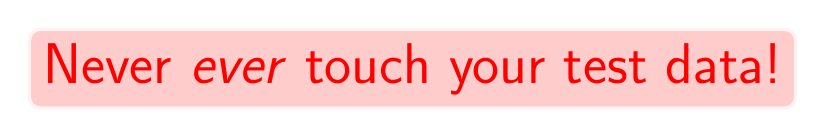
\begin{tikzpicture}[transform shape, rotate=0]
  \node [draw=Red!5, fill=Red!20, very thick, rectangle, rounded corners, inner sep=5pt, inner ysep=5pt] (box) {
    \textcolor{red}{\textsf{\huge Never \emph{ever} touch your test data!}}
  };
\end{tikzpicture}

If there is only one thing you learn from this book, let it be that.
Do not look at your test data.  Even once.  Even a tiny peek.  Once
you do that, it is not test data any more.  Yes, perhaps your
algorithm hasn't seen it.  But you have.  And you are likely a better
learner than your learning algorithm.  Consciously or otherwise, you
might make decisions based on whatever you might have seen.  Once you
look at the test data, your model's performance on it is no longer
indicative of it's performance on future unseen data.  This is simply
because future data is unseen, but your ``test'' data no longer is.

\section{Models, Parameters and Hyperparameters}

The general approach to machine learning, which captures many existing
learning algorithms, is the \concept{modeling} approach.  The idea is
that we come up with some formal model of our data.  For instance, we
might model the classification decision of a student/course pair as a
decision tree.  The choice of using a \emph{tree} to represent this
model is \emph{our choice.}  We also could have used an arithmetic
circuit or a polynomial or some other function.  The model tells us
what sort of things we can learn, and also tells us what our inductive
bias is.

For most models, there will be associated parameters.  These are the
things that we use the data to decide on.  Parameters in a decision
tree include: the specific questions we asked, the order in which we
asked them, and the classification decisions at the leaves.  The job
of our decision tree learning algorithm \FUN{DecisionTreeTrain} is to take data
and figure out a good set of parameters.

Many learning algorithms will have additional knobs that you can
adjust.  In most cases, these knobs amount to tuning the inductive
bias of the algorithm.  In the case of the decision tree, an obvious
knob that one can tune is the \concept{maximum depth} of the decision
tree.  That is, we could modify the \FUN{DecisionTreeTrain} function so that it
\emph{stops} recursing once it reaches some pre-defined maximum depth.
By playing with this depth knob, we can adjust between underfitting
(the empty tree, depth$=0$) and overfitting (the full tree,
depth$=\infty$).

\thinkaboutit{Go back to the \FUN{DecisionTreeTrain} algorithm and modify it so
  that it takes a maximum depth parameter.  This should require adding
  two lines of code and modifying three others.}

Such a knob is called a \concept{hyperparameter}.  It is so called
because it is a parameter that controls other parameters of the model.
The exact definition of hyperparameter is hard to pin down: it's one
of those things that are easier to identify than define.  However, one
of the key identifiers for hyperparameters (and the main reason that
they cause consternation) is that they cannot be naively adjusted
using the training data.

In \FUN{DecisionTreeTrain}, as in most machine learning, the learning algorithm
is essentially trying to adjust the parameters of the model so as to
minimize training error.  This suggests an idea for choosing
hyperparameters: choose them so that they minimize training error.

What is wrong with this suggestion?  Suppose that you were to treat
``maximum depth'' as a hyperparameter and tried to tune it on your
training data.  To do this, maybe you simply build a collection of
decision trees, tree$_0$, tree$_1$, tree$_2$, $\dots$, tree$_{100}$,
where tree$_d$ is a tree of maximum depth $d$.  We then computed the
training error of each of these trees and chose the ``ideal'' maximum
depth as that which minimizes training error?  Which one would it
pick?

The answer is that it would pick $d=100$.  Or, in general, it would
pick $d$ as large as possible.  Why?  Because choosing a bigger $d$
will \emph{never hurt} on the training data.  By making $d$ larger,
you are simply encouraging overfitting.  But by evaluating on the
training data, overfitting actually looks like a good idea!

An alternative idea would be to tune the maximum depth on test data.
This is promising because test data peformance is what we really want
to optimize, so tuning this knob on the test data seems like a good
idea.  That is, it won't accidentally reward overfitting.  Of course,
it breaks our cardinal rule about test data: that you should never
touch your test data.  So that idea is immediately off the table.

However, our ``test data'' wasn't magic.  We simply took our $1000$
examples, called $800$ of them ``training'' data and called the other
$200$ ``test'' data.  So instead, let's do the following.  Let's take
our original $1000$ data points, and select $700$ of them as training
data.  From the remainder, take $100$ as \concept{development
  data}\sidenote{Some people call this ``\concept{validation data}''
  or ``\concept{held-out data}.''} and the remaining $200$ as test
data.  The job of the development data is to allow us to tune
hyperparameters.  The general approach is as follows:

\begin{enumerate}
\item Split your data into $70\%$ training data, $10\%$ development
  data and $20\%$ test data.

\item For each possible setting of your hyperparameters:

\begin{enumerate}
\item Train a model using that setting of hyperparameters on the
  training data.

\item Compute this model's error rate on the development data.
\end{enumerate}

\item From the above collection of models, choose the one that
  achieved the lowest error rate on development data.

\item Evaluate that model on the test data to estimate future test
  performance.
\end{enumerate}

\thinkaboutit{In step 3, you could either choose the model (trained on
  the $70\%$ training data) that did the best on the development data.
  Or you could choose the hyperparameter settings that did best and
  \emph{retrain} the model on the $80\%$ union of training and
  development data.  Is either of these options obviously better or
  worse?}

\section{Chapter Summary and Outlook}

At this point, you should be able to use decision trees to do machine
learning.  Someone will give you data.  You'll split it into
training, development and test portions.  Using the training and
development data, you'll find a good value for maximum depth that
trades off between underfitting and overfitting.  You'll then run the
resulting decision tree model on the test data to get an estimate of
how well you are likely to do in the future.

You might think: why should I read the rest of this book?  Aside from
the fact that machine learning is just an awesome fun field to learn
about, there's a lot left to cover.  In the next two chapters, you'll
learn about two models that have very different inductive biases than
decision trees.  You'll also get to see a very useful way of thinking
about learning: the geometric view of data.  This will guide much of
what follows.  After that, you'll learn how to solve problems more
complicated that simple binary classification.  (Machine learning
people like binary classification a lot because it's one of the
simplest non-trivial problems that we can work on.)  After that,
things will diverge: you'll learn about ways to think about learning
as a formal optimization problem, ways to speed up learning, ways to
learn without labeled data (or with very little labeled data) and all
sorts of other fun topics.

But throughout, we will focus on the view of machine learning that
you've seen here.  You select a model (and its associated inductive
biases).  You use data to find parameters of that model that work well
on the training data.  You use development data to avoid underfitting
and overfitting.  And you use test data (which you'll never look at or
touch, right?) to estimate future model performance.  Then you conquer
the world.

%\section{Decision Trees with Real-Valued Features}

\begin{comment}
Predicting the future
 - Not memorizing the past (simple prediction problem)
 - Generalizing from known to unknown
 - Training versus test data

Models, algorithms, theory and experiments

Evaluation

Optimizing 0/1 loss

Underfitting/overfitting by depth

Pruning

From two classes to M classes
\end{comment}

\begin{exercises}
\begin{Ex}
\TODO

\begin{solution}
\TODO
\end{solution}
\end{Ex}

\end{exercises}

%%% Local Variables: 
%%% mode: latex
%%% TeX-master: "courseml"
%%% End: 
